\chapter{Jade e Jason}

\section{Jade}

\subsection{FIPA}

\dfn{FIPA}{
  Consorzio per la standardizzazione di sistemi ad agenti. Il suo obiettivo era quello di promuovere tecnologie interoperabili: sistemi di agenti intelligenti che lavorano insieme.
}

\qs{}{Cosa rientrà nelle competenze di FIPA?}

\begin{itemize}
  \item Gestione del ciclo di vita di un agente. 
  \item Come trasportare un messaggio. 
  \item La struttura di un messaggio. 
  \item Protocolli di interazione tra agenti. 
  \item Ontologie e sicurezza.
\end{itemize}

\nt{Gli agenti sono al di fuori degli obiettivi di FIPA.}

\paragraph{Caratteristiche che vengono assunte per gli agenti:}

\begin{itemize}
  \item Autonomi. 
  \item Reattivi. 
  \item Proattivi. 
  \item Goal-driven. 
  \item Sociali. 
  \item Adattivi. 
  \item Cognitivi.
\end{itemize}

\begin{figure}[!h]
    \centering
    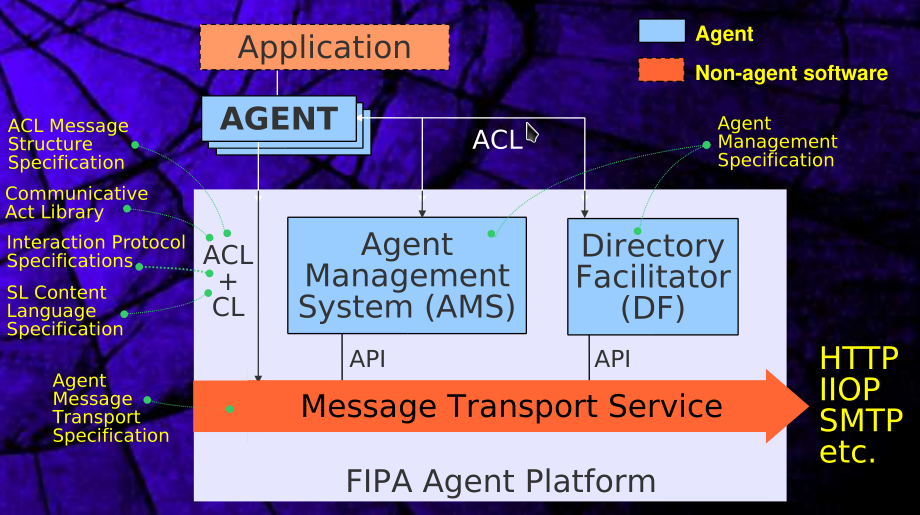
\includegraphics[scale=0.35]{05/FIPA.png}
  \caption{Piattaforma FIPA per agenti.}
\end{figure}

\cor{Agent Management}{
  Gli agenti hanno una descrizione di sé stessi e dei servizi che vengono offerti. L'Agent Management sistem è a sua volta un agente con cui si interagisce con scambi di messaggi. In jade si può accedere così oppure accedere direttamente agli oggetti Java.
}

\begin{figure}[!h]
    \centering
    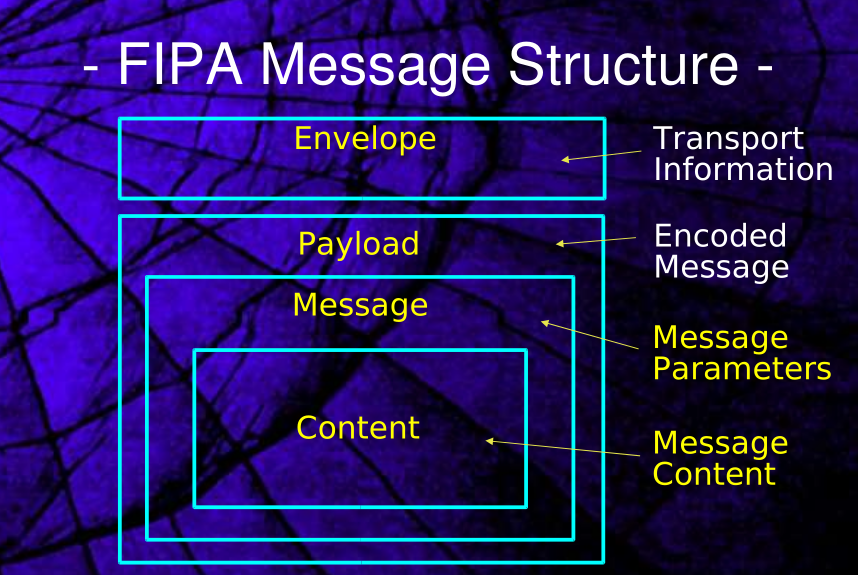
\includegraphics[scale=0.35]{05/messaggi.png}
  \caption{Specifica per i messaggi.}
\end{figure}

\subsection{Introduzione a JADE}

\qs{}{Che cos'è JADE?}

\paragraph{Risposta:} JADE è la piattaforma, all'interno del consorzio FIPA, che implementa lo standard sopra citato. Si presenta come codice Java puro. Offre una serie di librerie per agenti e un runtime envinronment per gli agenti creati. L'obiettivo è quello di "nascondere" FIPA al programmatore. 

\begin{figure}[!h]
    \centering
    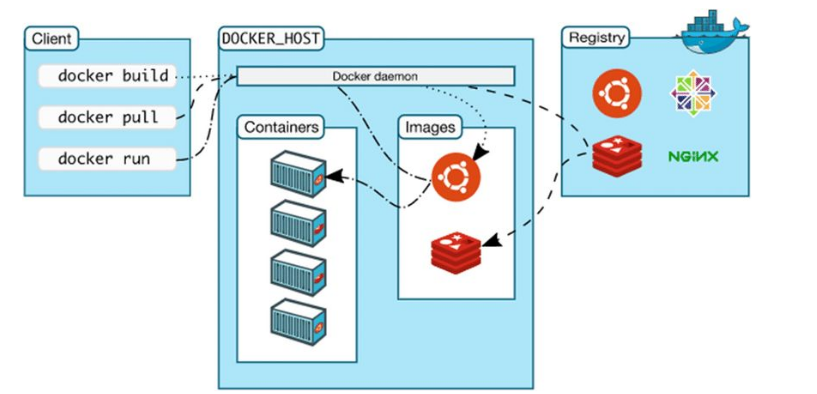
\includegraphics[scale=0.45]{05/arch.png}
  \caption{Modello architetturale di JADE.}
\end{figure}


\section{Jason}
